\documentclass[tikz,border=2pt]{standalone}
\usepackage{tikz}
\usepackage{lmodern}
\usetikzlibrary{calc,decorations.pathreplacing}

% Visual conventions follow the existing MRNC TikZ pictures: ordinary
% components use TikZ's normal 0.4pt stroke, with compact TeX labels.
\tikzset{
  nu fibre/.style={
    x=0.78cm,
    y=0.78cm,
    line width=0.4pt,
    line cap=round,
    line join=round
  },
  nu label/.style={
    font=\scriptsize,
    inner sep=1pt
  },
  nu annotation/.style={
    font=\scriptsize,
    inner sep=1pt
  },
  nu dots/.style={
    font=\small,
    inner sep=0pt
  }
}

\begin{document}

%IV-II_0
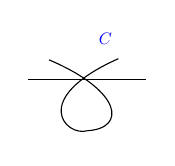
\begin{tikzpicture}[scale=0.5]
  % Coordinates
  \coordinate (A) at (-1.50, 2.00);
  \coordinate (B) at (1.50, 2.00);
  \coordinate (C) at (-0.00, 0.69);
  \coordinate (D) at (-0.97, 2.49);
  \coordinate (E) at (1.00, 0.75);
  \coordinate (F) at (0.89, 1.70);
  \coordinate (G) at (0.79, 2.52);
  \coordinate (H) at (-0.53, 0.53);
  \coordinate (I) at (-1.50, 1.50);
  \coordinate (G_1) at (0.46, 2.73);

  % Drawing
  \draw (A) -- (B);
  \draw (C) .. controls (1.00, 0.75) and (0.89, 1.70) .. (D);
  \draw (C) .. controls (-0.53, 0.53) and (-1.50, 1.50) .. (G);
  \node[scale=0.6][above, text=blue] at (G_1) {$C$};
\end{tikzpicture}


\end{document}
